\documentclass{report}

\usepackage{hyperref}

\usepackage{epstopdf}
\usepackage{amsmath}
\usepackage{amssymb}
\usepackage{subfig}
%\usepackage{multirow}
\usepackage[utf8]{inputenc}
\usepackage[T1]{fontenc}
\usepackage{standalone}
\usepackage{tikz}
\usepackage{tabularx}
\usepackage{float}
\usepackage[section]{placeins}
\usepackage{sverb}
\usepackage{import}
\usepackage{verbatim}
\usepackage{listings}
\usepackage{xcolor}

\graphicspath{{img/}}
\DeclareGraphicsExtensions{.pdf,.png,.jpg,.svg} %For pdflatex






\definecolor{codegreen}{rgb}{0,0.6,0}
\definecolor{codegray}{rgb}{0.5,0.5,0.5}
\definecolor{codepurple}{rgb}{0.58,0,0.82}
\definecolor{backcolour}{rgb}{0.95,0.95,0.92}

\lstdefinestyle{mystyle}{
    backgroundcolor=\color{backcolour},   
    commentstyle=\color{codegreen},
    keywordstyle=\color{magenta},
    numberstyle=\tiny\color{codegray},
    stringstyle=\color{codepurple},
    basicstyle=\ttfamily\footnotesize,
    breakatwhitespace=false,         
    breaklines=true,                 
    captionpos=b,                    
    keepspaces=true,                 
    numbers=left,                    
    numbersep=5pt,                  
    showspaces=false,                
    showstringspaces=false,
    showtabs=false,                  
    tabsize=2,
    float=H,
    extendedchars=\true, 
}


\lstset{style=mystyle}


\begin{document}

\begin{titlepage}
    \begin{center}
        
\includegraphics[width=.50\linewidth]{other/polsl.png}\\
        \Huge
        \textbf{Przetwarzanie Obrazów Cyfrowych}
        \\ \vspace{1.5cm}
        \Large
        \textbf{Raport z ćwiczenia nr. 6: } \\
        % \textbf{WSTĘPNE PRZETWARZANIE OBRAZÓW — FILTRY LINIOWE}
        \textbf{Wstępne przetwarzanie obrazów - filtry liniowe}        
    \end{center}
    \vspace{3.0cm}
    \Large
    Raport opracował: \\
    Dawid Kania \\
    Grupa 6 Semestr 6 \\ \\
    Data wykonania ćwiczenia: 09.06.2022
\end{titlepage}
 


\section*{Zadanie 1. Operacje na histogramach}
\subsection*{Rozciąganie histogramu}


\newcommand{\ww}{0.33}
\begin{figure}[H]
    \captionsetup[subfloat]{justification=raggedright,singlelinecheck=false, position=bottom,labelformat=empty} %
    \subfloat[Ox           ]{\includegraphics[width=\ww\linewidth]{../zad1/NoCut/I1/I_Origin.png}} \hfill%	
    \subfloat[HS(Ox)       ]{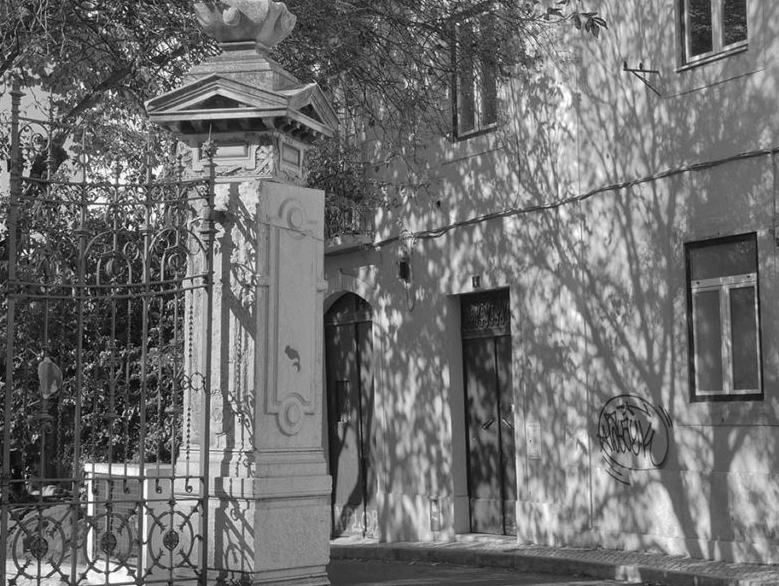
\includegraphics[width=\ww\linewidth]{../zad1/NoCut/I1/I_No_Cut.png}} \hfill% wypełnenie
    \subfloat[HE(Ox)       ]{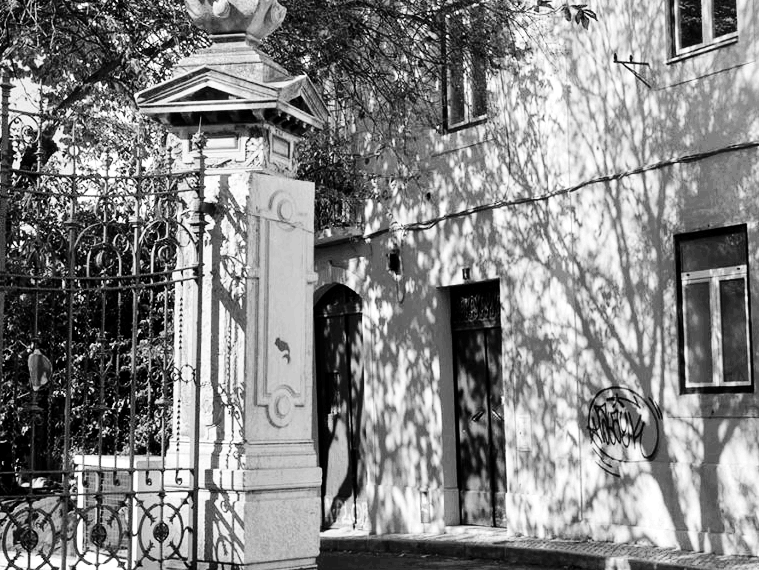
\includegraphics[width=\ww\linewidth]{../zad1/NoCut/I1/I_Histeq.png}} \\
    \subfloat[H(Ox)     \\ k1 = 0.28627 \\ k2 = 2.3275 \\ k3 = 1 \\ k4 = 0.010884 \\ min(I) = 0 \\ max(I) = 0.28627 ]{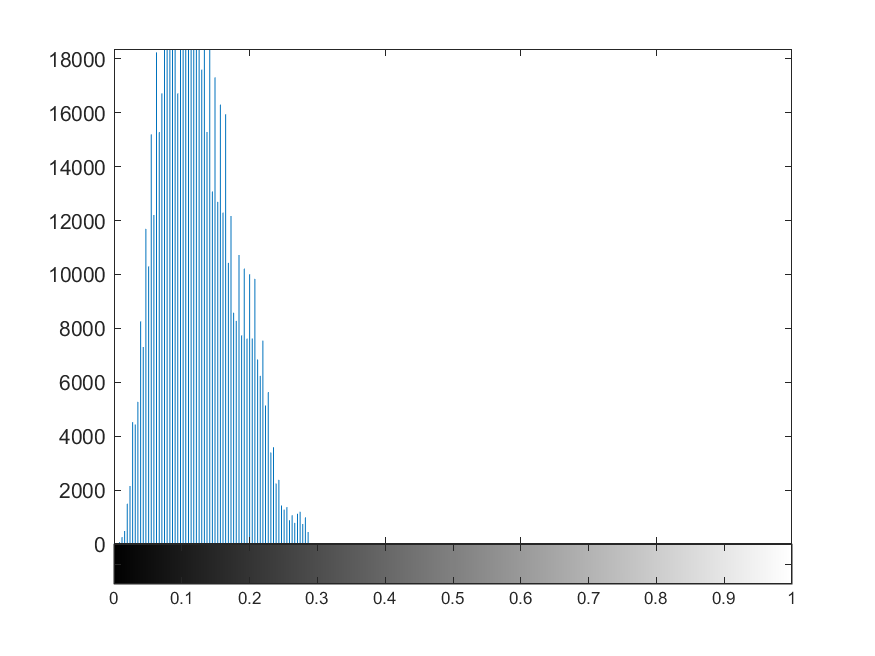
\includegraphics[width=\ww\linewidth]{../zad1/NoCut/I1/H_Origin.png}} \hfill%	
    \subfloat[H(HS(Ox)) \\ k1 = 1 \\ k2 = 2.3275 \\ k3 = 1 \\ k4 = 0.13281 \\ min(I) = 0 \\ max(I) = 1 ]{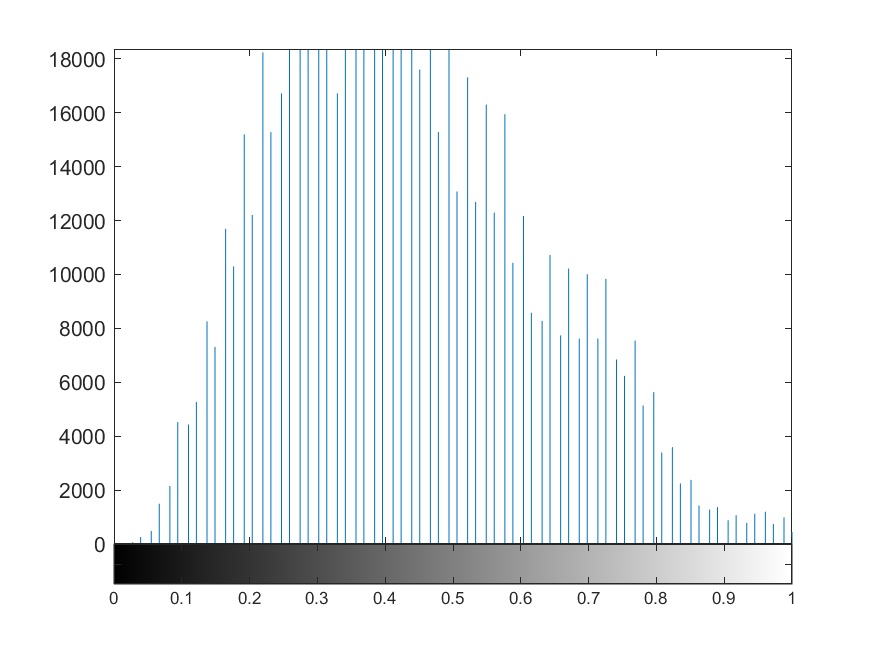
\includegraphics[width=\ww\linewidth]{../zad1/NoCut/I1/H_No_Cut.png}} \hfill
    \subfloat[H(HE(Ox)) \\ k1 = 1 \\ k2 = 2.0034 \\ k3 = 1 \\ k4 = 0.34362 \\ min(I) = 0 \\ max(I) = 1 ]{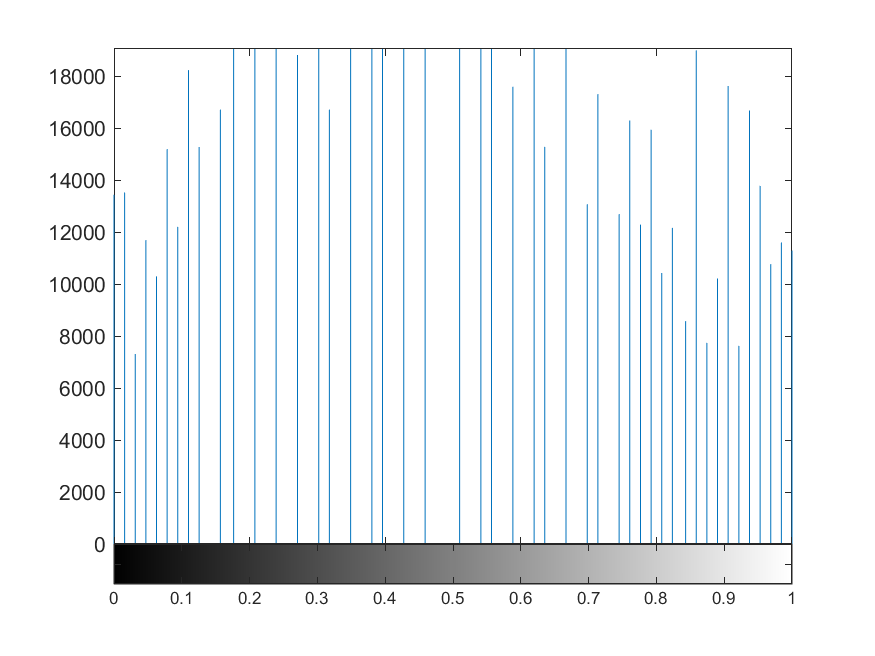
\includegraphics[width=\ww\linewidth]{../zad1/NoCut/I1/H_Histeq.png}} 
    \caption{Tekst do zmiany} 
    \label{fig:porownanie1}
\end{figure}

\begin{figure}[H]
    \captionsetup[subfloat]{justification=raggedright,singlelinecheck=false, position=bottom,labelformat=empty} %
    \subfloat[Ox           ]{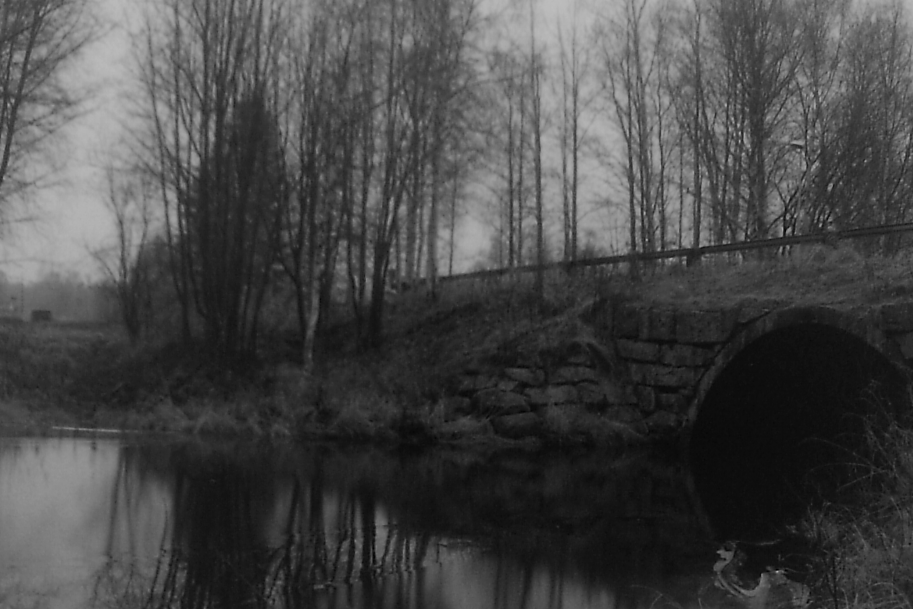
\includegraphics[width=\ww\linewidth]{../zad1/NoCut/I2/I_Origin.png}} \hfill%	
    \subfloat[HS(Ox)       ]{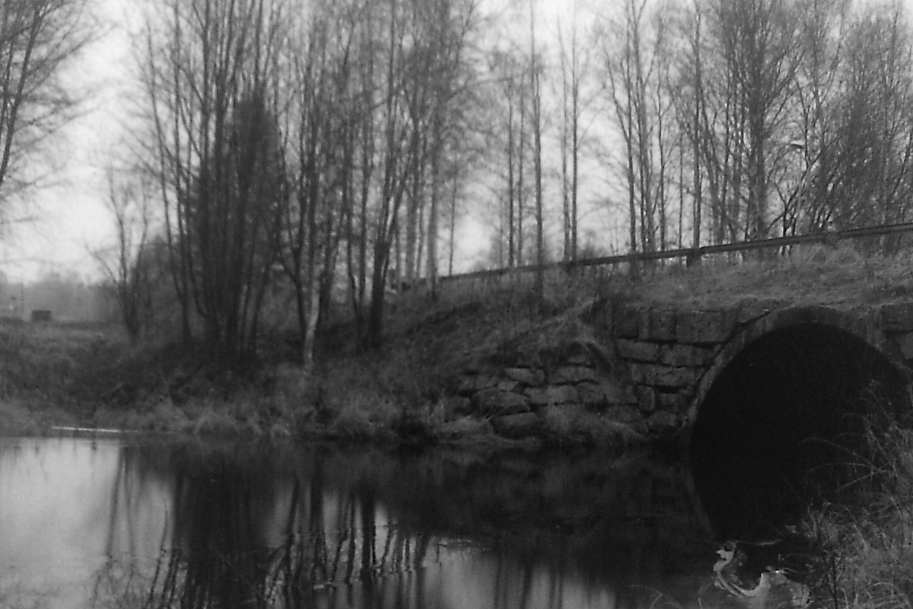
\includegraphics[width=\ww\linewidth]{../zad1/NoCut/I2/I_No_Cut.png}} \hfill% wypełnenie
    \subfloat[HE(Ox)       ]{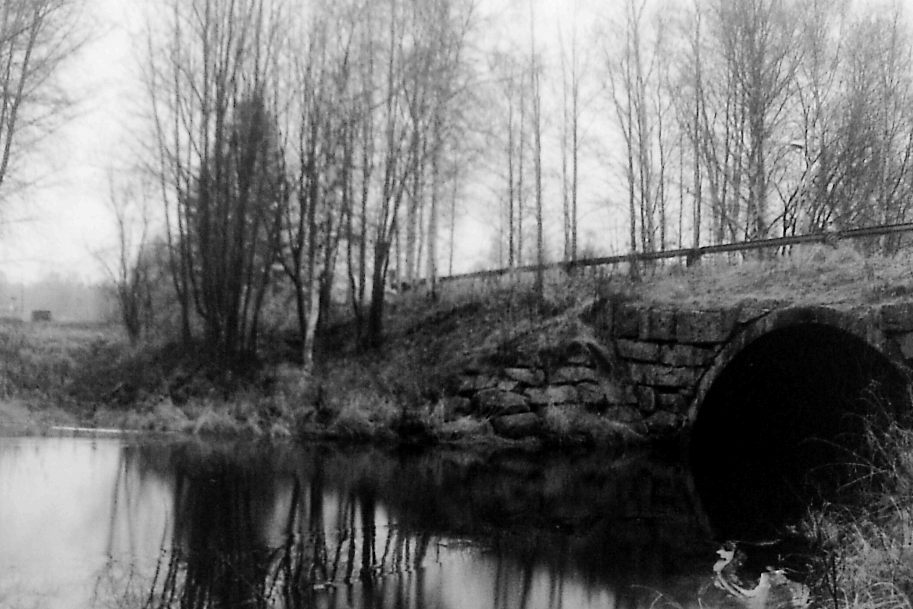
\includegraphics[width=\ww\linewidth]{../zad1/NoCut/I2/I_Histeq.png}} \\
    \subfloat[H(Ox)     \\ k1 = 0.76078 \\ k2 = 2.4201 \\ k3 = 1 \\ k4 = 0.15035 \\ min(I) = 0 \\ max(I) = 0.76078 ]{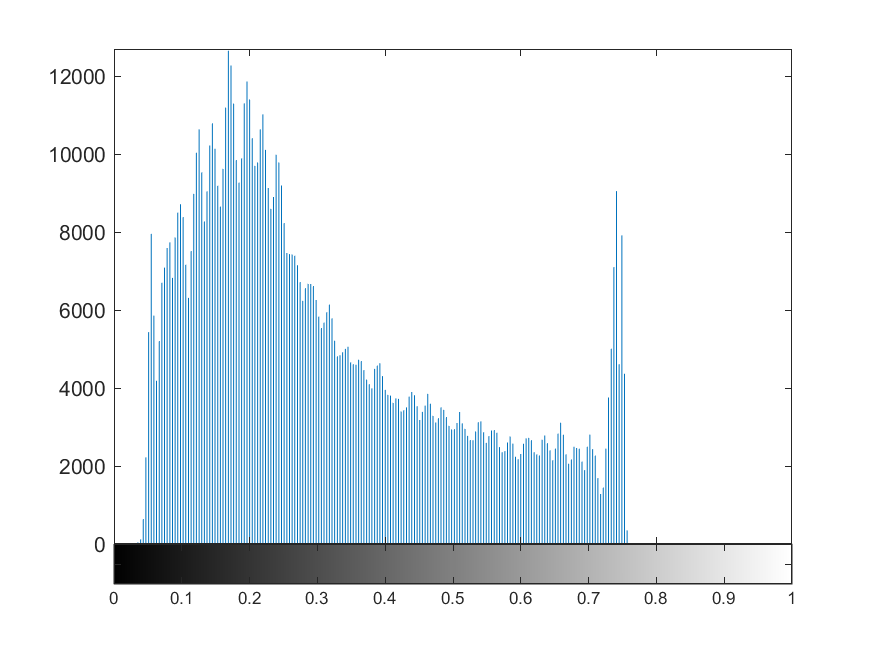
\includegraphics[width=\ww\linewidth]{../zad1/NoCut/I2/H_Origin.png}} \hfill%	
    \subfloat[H(HS(Ox)) \\ k1 = 1 \\ k2 = 2.4201 \\ k3 = 1 \\ k4 = 0.25977 \\ min(I) = 0 \\ max(I) = 1 ]{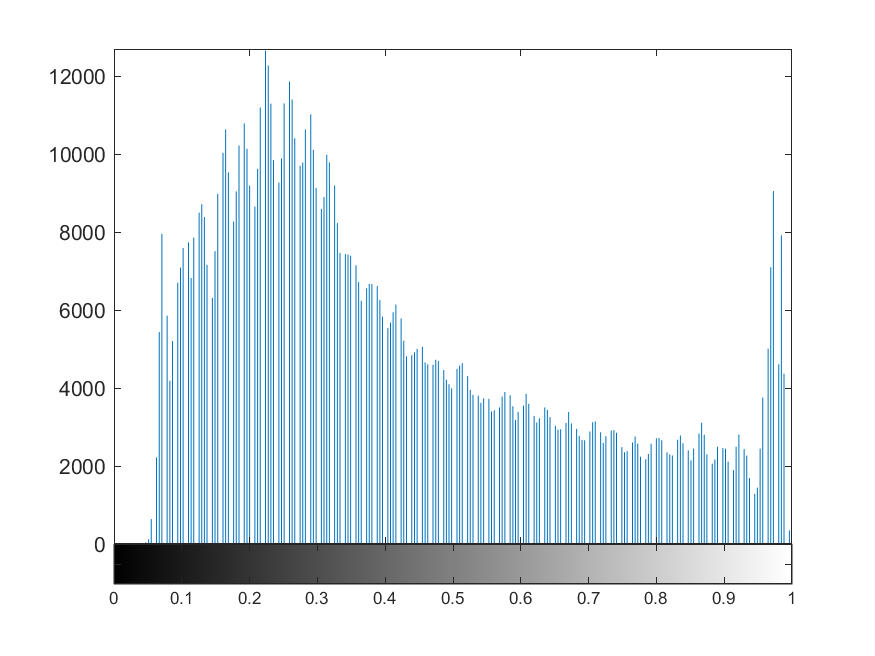
\includegraphics[width=\ww\linewidth]{../zad1/NoCut/I2/H_No_Cut.png}} \hfill
    \subfloat[H(HE(Ox)) \\ k1 = 1 \\ k2 = 2.001 \\ k3 = 1 \\ k4 = 0.34525 \\ min(I) = 0 \\ max(I) = 1 ]{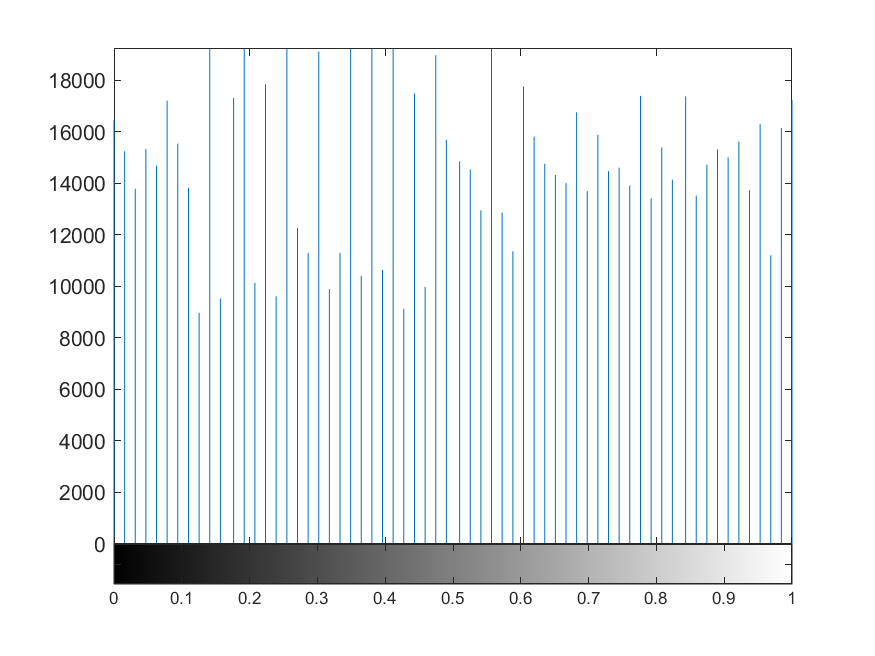
\includegraphics[width=\ww\linewidth]{../zad1/NoCut/I2/H_Histeq.png}} 
    \caption{Tekst do zmiany} 
    \label{fig:porownanie2}
\end{figure}

\begin{figure}[H]
    \captionsetup[subfloat]{justification=raggedright,singlelinecheck=false, position=bottom,labelformat=empty} %
    \subfloat[Ox           ]{\includegraphics[width=\ww\linewidth]{../zad1/NoCut/I3/I_Origin.png}} \hfill%	
    \subfloat[HS(Ox)       ]{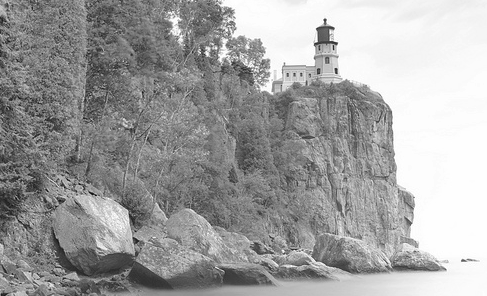
\includegraphics[width=\ww\linewidth]{../zad1/NoCut/I3/I_No_Cut.png}} \hfill% wypełnenie
    \subfloat[HE(Ox)       ]{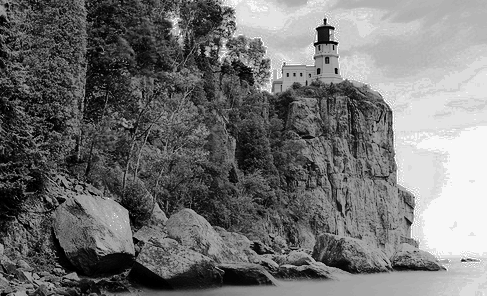
\includegraphics[width=\ww\linewidth]{../zad1/NoCut/I3/I_Histeq.png}} \\
    \subfloat[H(Ox)     \\ k1 = 0.81961 \\ k2 = 1.479 \\ k3 = 1 \\ k4 = 0.16253 \\ min(I) = 0 \\ max(I) = 0.81961 ]{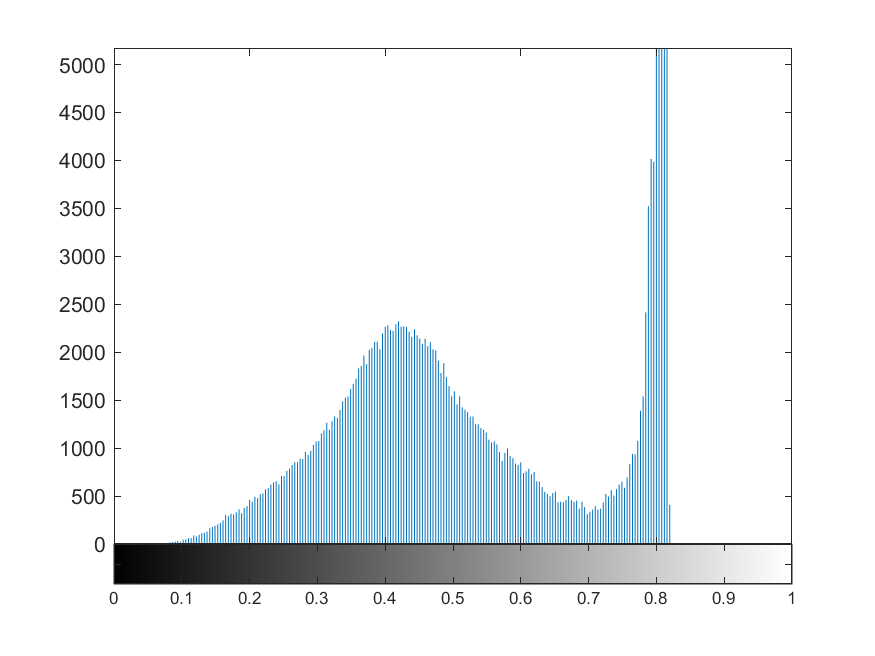
\includegraphics[width=\ww\linewidth]{../zad1/NoCut/I3/H_Origin.png}} \hfill%	
    \subfloat[H(HS(Ox)) \\ k1 = 1 \\ k2 = 1.479 \\ k3 = 1 \\ k4 = 0.24194 \\ min(I) = 0 \\ max(I) = 1 ]{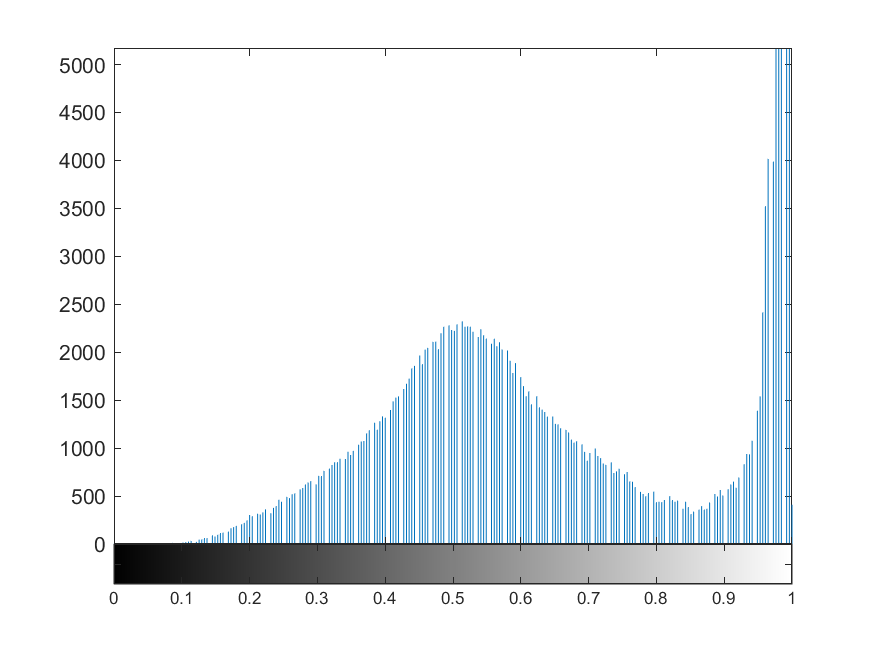
\includegraphics[width=\ww\linewidth]{../zad1/NoCut/I3/H_No_Cut.png}} \hfill
    \subfloat[H(HE(Ox)) \\ k1 = 1 \\ k2 = 1.9995 \\ k3 = 1 \\ k4 = 0.34542 \\ min(I) = 0 \\ max(I) = 1 ]{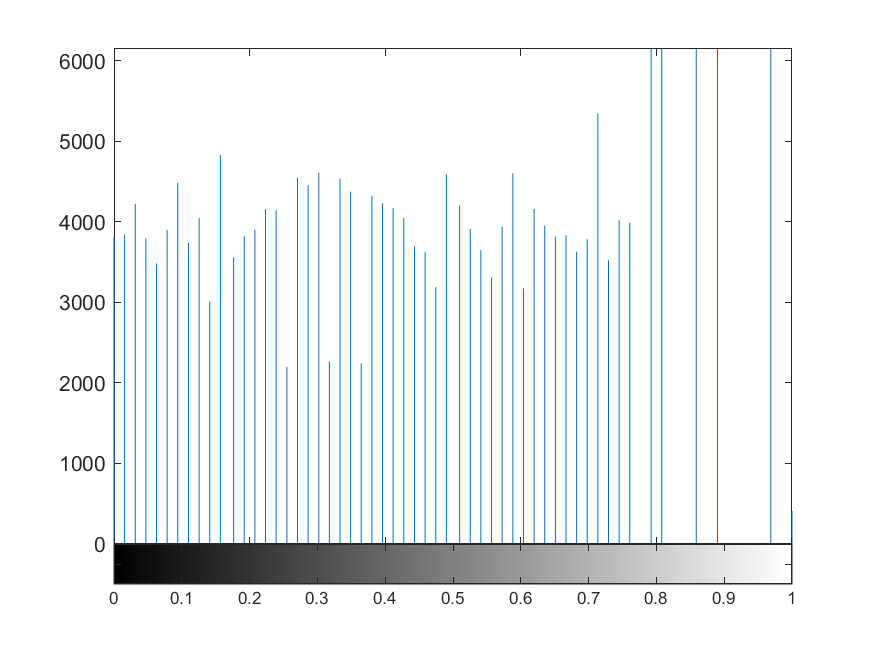
\includegraphics[width=\ww\linewidth]{../zad1/NoCut/I3/H_Histeq.png}} 
    \caption{Tekst do zmiany} 
    \label{fig:porownanie3}
\end{figure}

\begin{figure}[H]
    \captionsetup[subfloat]{justification=raggedright,singlelinecheck=false, position=bottom,labelformat=empty} %
    \subfloat[Ox           ]{\includegraphics[width=\ww\linewidth]{../zad1/NoCut/I4/I_Origin.png}} \hfill%	
    \subfloat[HS(Ox)       ]{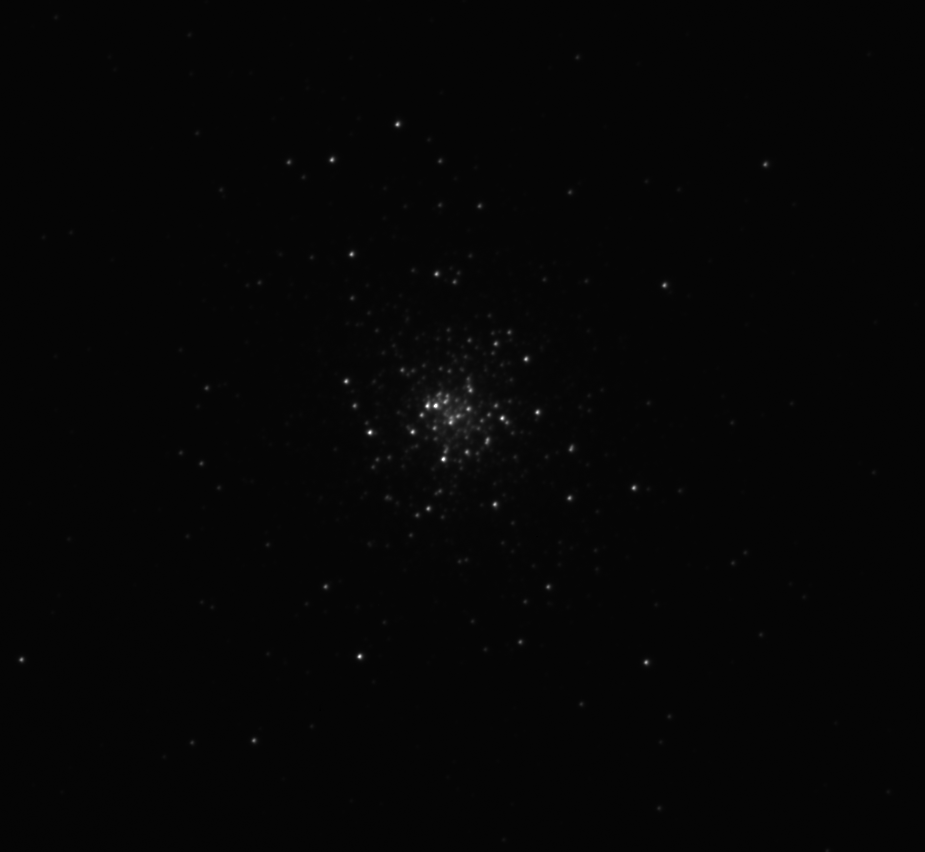
\includegraphics[width=\ww\linewidth]{../zad1/NoCut/I4/I_No_Cut.png}} \hfill% wypełnenie
    \subfloat[HE(Ox)       ]{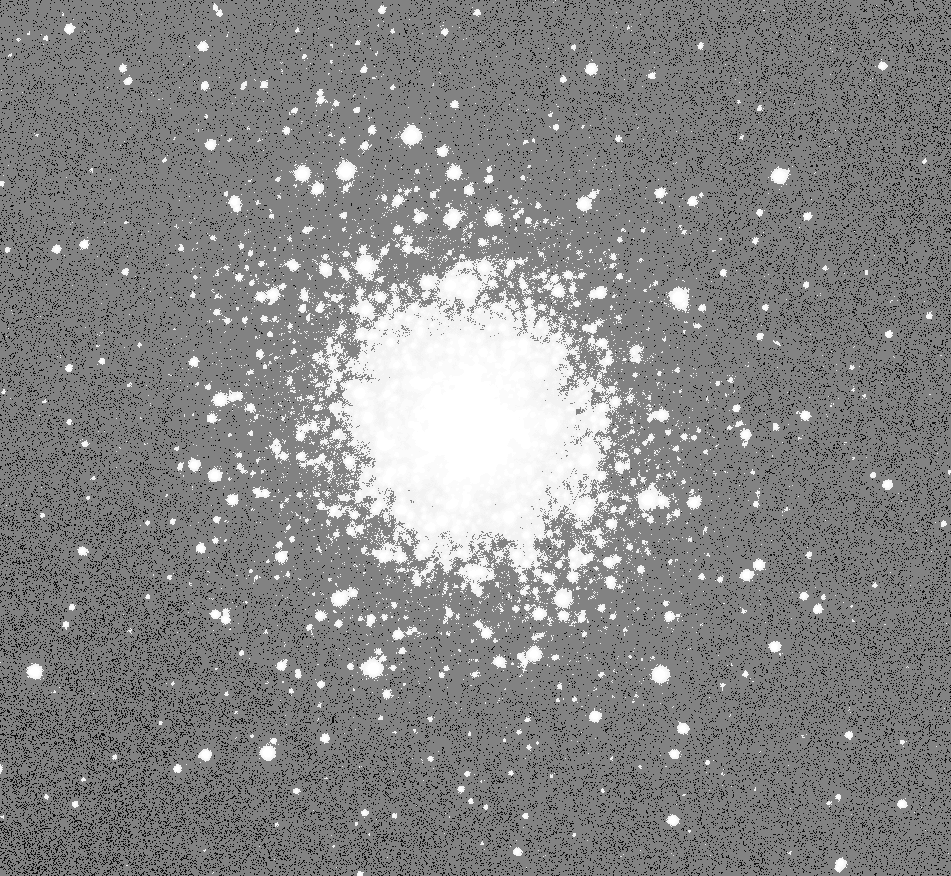
\includegraphics[width=\ww\linewidth]{../zad1/NoCut/I4/I_Histeq.png}} \\
    \subfloat[H(Ox)     \\ k1 = 0.99216 \\ k2 = 31.319 \\ k3 = 0.98444 \\ k4 = 0.013196 \\ min(I) = 0.0078431 \\ max(I) = 1 ]{\includegraphics[width=\ww\linewidth]{../zad1/NoCut/I4/H_Origin.png}} \hfill%	
    \subfloat[H(HS(Ox)) \\ k1 = 1 \\ k2 = 41.625 \\ k3 = 1 \\ k4 = 0.013405 \\ min(I) = 0 \\ max(I) = 1 ]{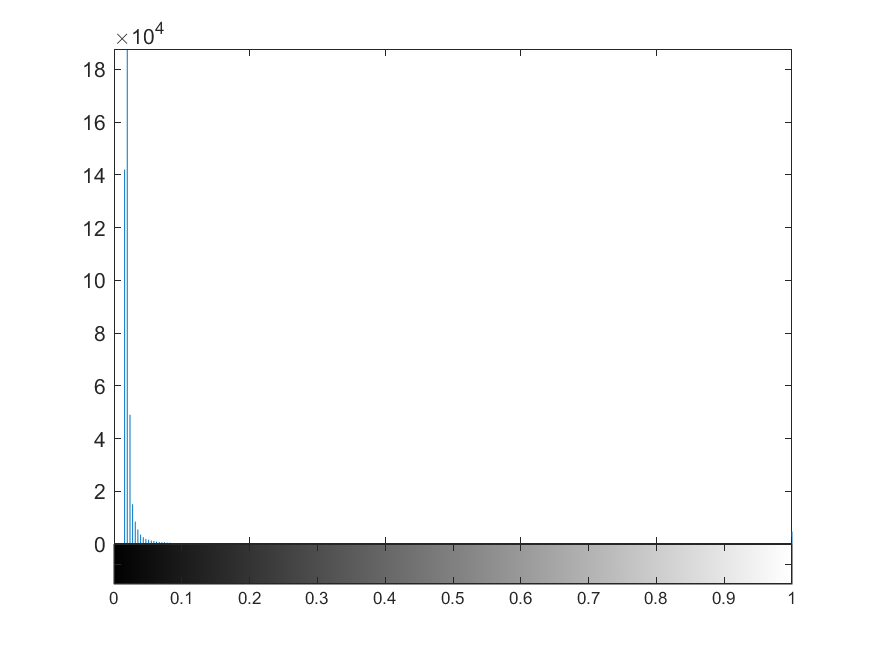
\includegraphics[width=\ww\linewidth]{../zad1/NoCut/I4/H_No_Cut.png}} \hfill
    \subfloat[H(HE(Ox)) \\ k1 = 1 \\ k2 = 2.0148 \\ k3 = 1 \\ k4 = 0.14579 \\ min(I) = 0 \\ max(I) = 1 ]{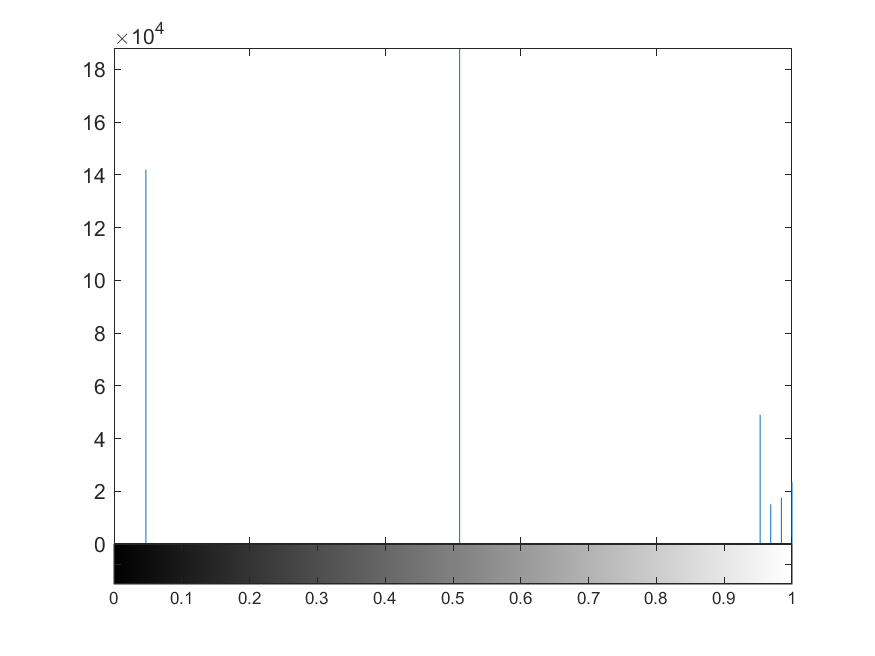
\includegraphics[width=\ww\linewidth]{../zad1/NoCut/I4/H_Histeq.png}} 
    \caption{Tekst do zmiany} 
    \label{fig:porownanie4}
\end{figure}



\subsection*{Rozciąganie histogramu z obcinaniem}

\begin{figure}[H]
    \captionsetup[subfloat]{justification=raggedright,singlelinecheck=false, position=bottom,labelformat=empty} %
    \subfloat[$\text{Ox}_\text{+b\&w}$                ]{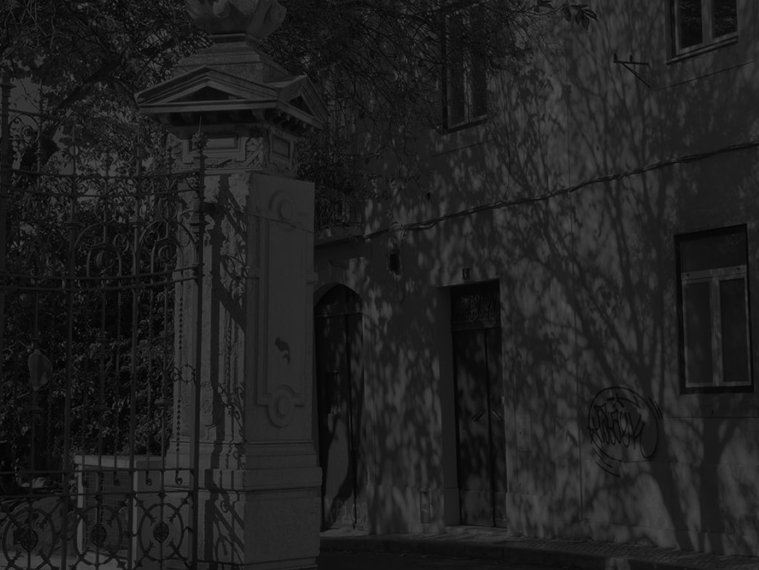
\includegraphics[width=\ww\linewidth]{../zad1/WithCut/I1/I_Origin.png}} \hfill%	
    \subfloat[HSc($\text{Ox}_\text{+b\&w}$ ,p1)       ]{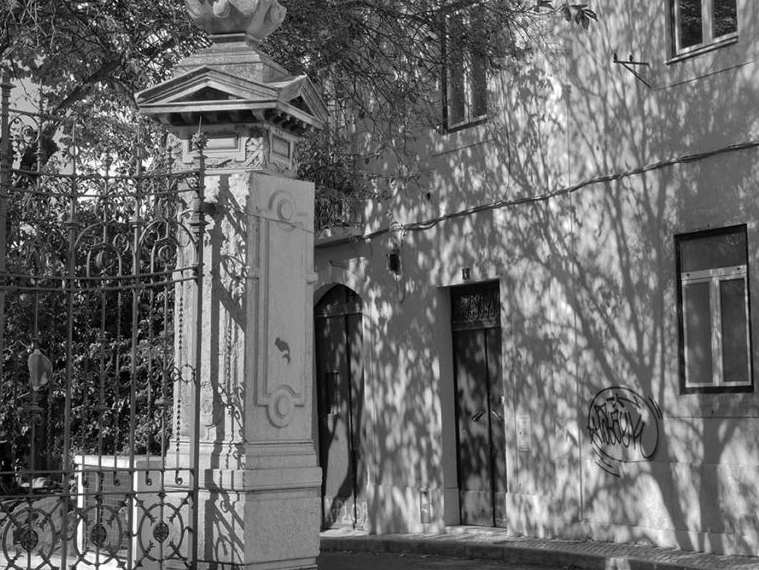
\includegraphics[width=\ww\linewidth]{../zad1/WithCut/I1/I_Cut_P1.png}} \hfill% wypełnenie
    \subfloat[HSc($\text{Ox}_\text{+b\&w}$ ,p1)       ]{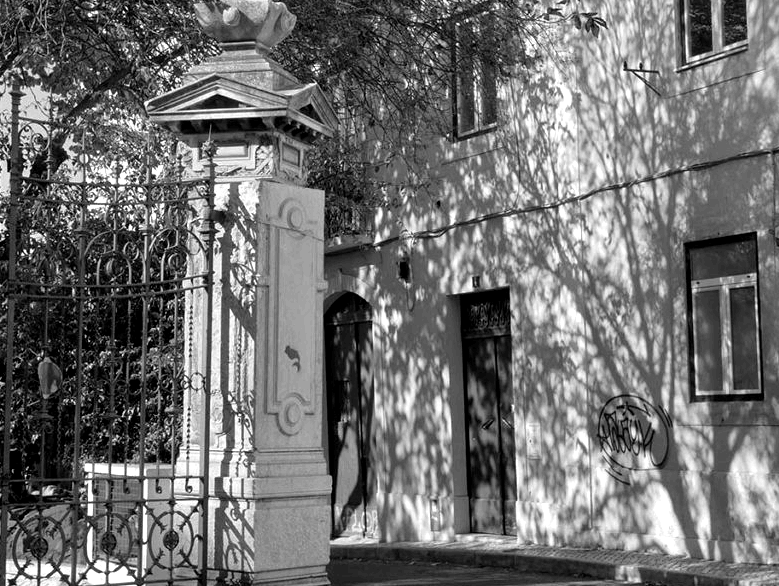
\includegraphics[width=\ww\linewidth]{../zad1/WithCut/I1/I_Cut_P2.png}} \\
    \subfloat[H($\text{Ox}_\text{+b\&w}$)          \\ k1 = 1 \\ k2 = 8.1303 \\ k3 = 1 \\ k4 = 0.010888 \\ min(I) = 0 \\ max(I) = 1 ]{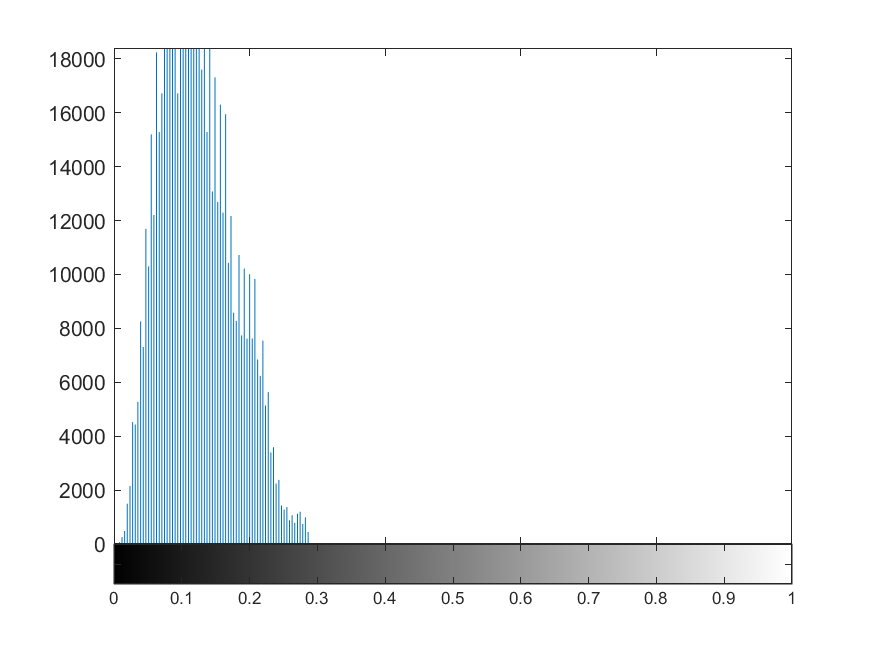
\includegraphics[width=\ww\linewidth]{../zad1/WithCut/I1/H_Origin.png}} \hfill%	
    \subfloat[H(HSc($\text{Ox}_\text{+b\&w}$ ,p1)) \\ k1 = 1 \\ k2 = 2.485 \\ k3 = 1 \\ k4 = 0.15298 \\ min(I) = 0 \\ max(I) = 1 ]{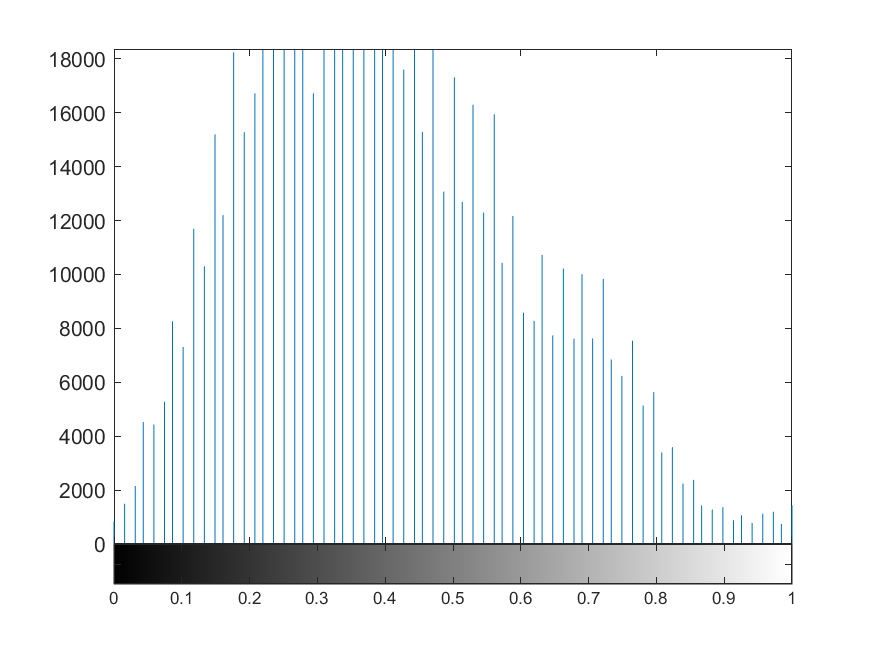
\includegraphics[width=\ww\linewidth]{../zad1/WithCut/I1/H_Cut_P1.png}} \hfill
    \subfloat[H(HSc($\text{Ox}_\text{+b\&w}$ ,p1)) \\ k1 = 1 \\ k2 = 2.3309 \\ k3 = 1 \\ k4 = 0.24966 \\ min(I) = 0 \\ max(I) = 1 ]{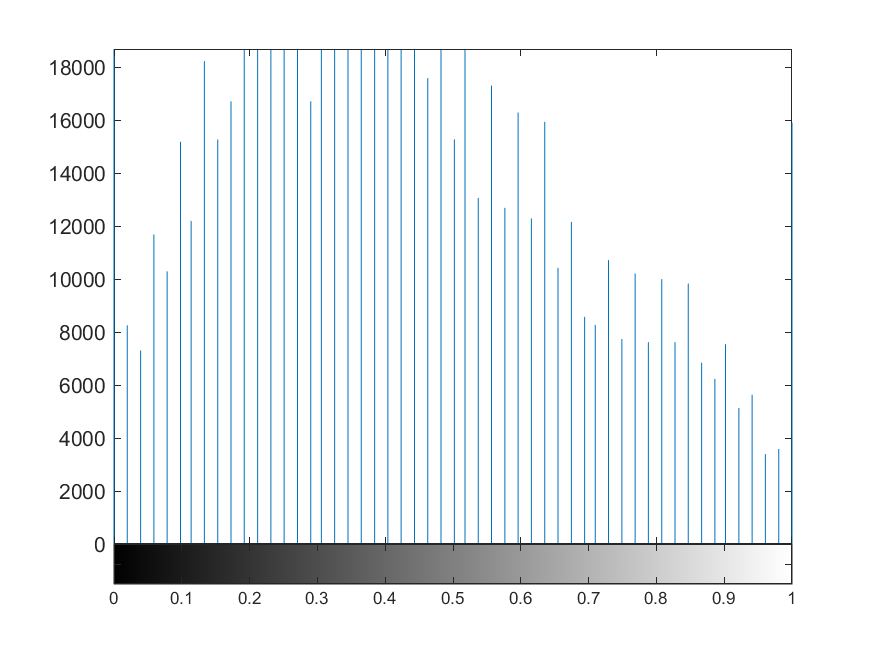
\includegraphics[width=\ww\linewidth]{../zad1/WithCut/I1/H_Cut_P2.png}} 
    \caption{Tekst do zmiany} 
    \label{fig:porownanie5}
\end{figure}

\begin{figure}[H]
    \captionsetup[subfloat]{justification=raggedright,singlelinecheck=false, position=bottom,labelformat=empty} %
    \subfloat[$\text{Ox}_\text{+b\&w}$                ]{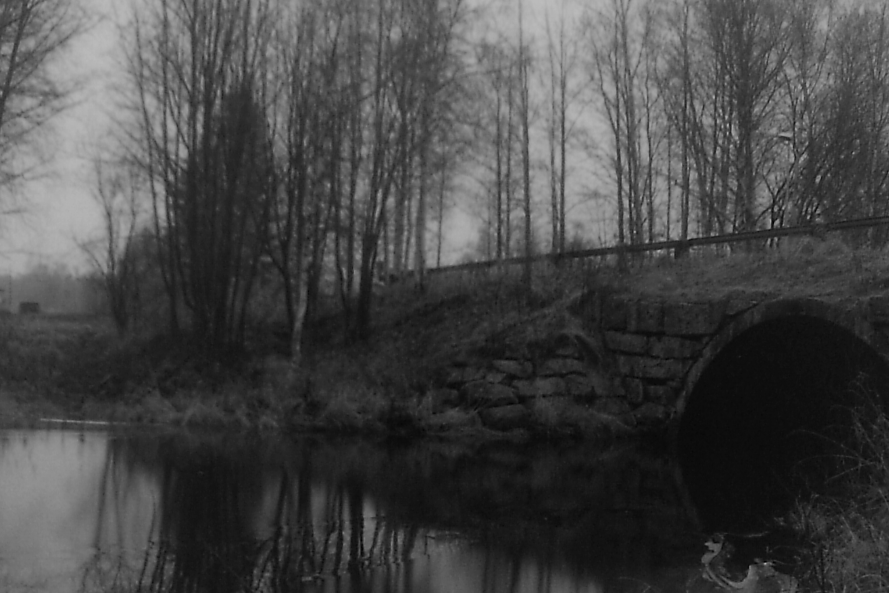
\includegraphics[width=\ww\linewidth]{../zad1/WithCut/I2/I_Origin.png}} \hfill%	
    \subfloat[HSc($\text{Ox}_\text{+b\&w}$ ,p1)       ]{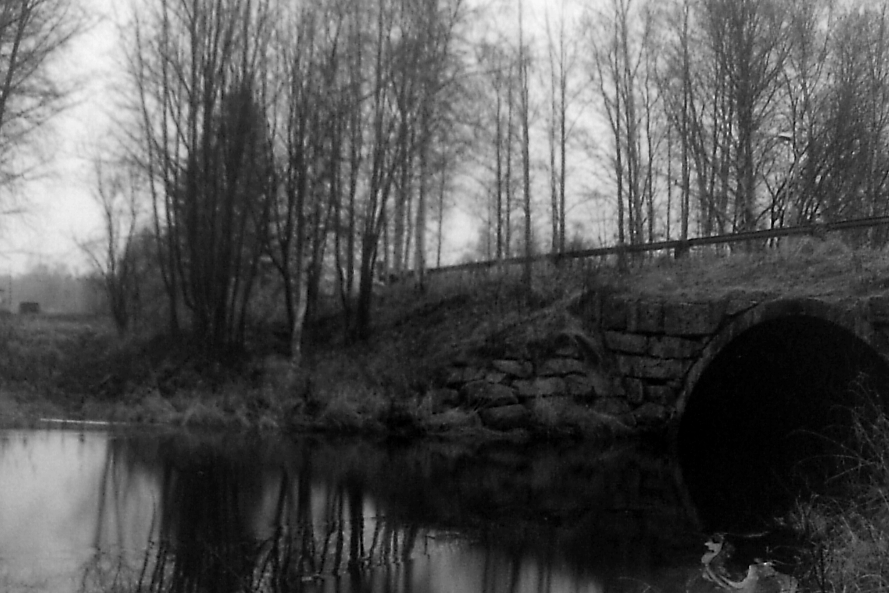
\includegraphics[width=\ww\linewidth]{../zad1/WithCut/I2/I_Cut_P1.png}} \hfill% wypełnenie
    \subfloat[HSc($\text{Ox}_\text{+b\&w}$ ,p1)       ]{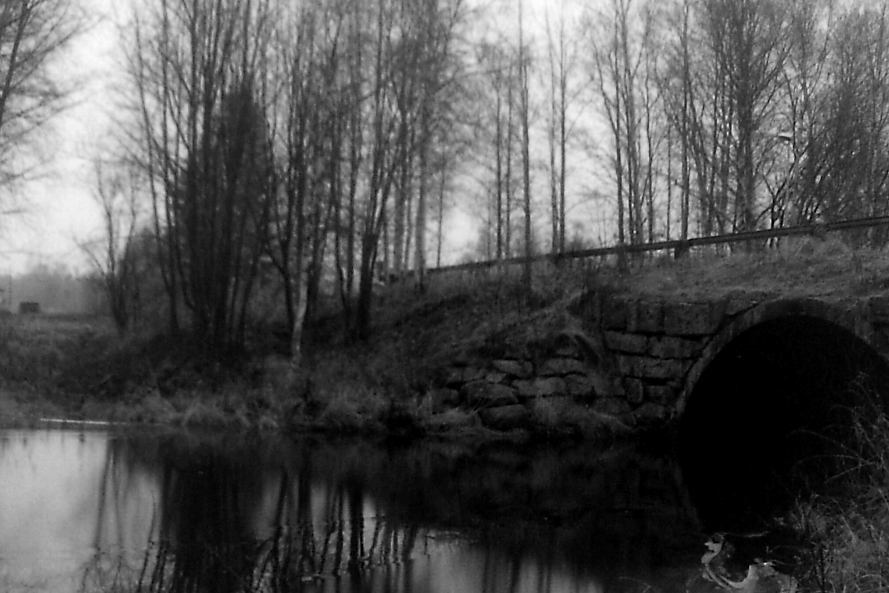
\includegraphics[width=\ww\linewidth]{../zad1/WithCut/I2/I_Cut_P2.png}} \\
    \subfloat[H($\text{Ox}_\text{+b\&w}$)          \\ k1 = 1 \\ k2 = 3.181 \\ k3 = 1 \\ k4 = 0.15035 \\ min(I) = 0 \\ max(I) = 1 ]{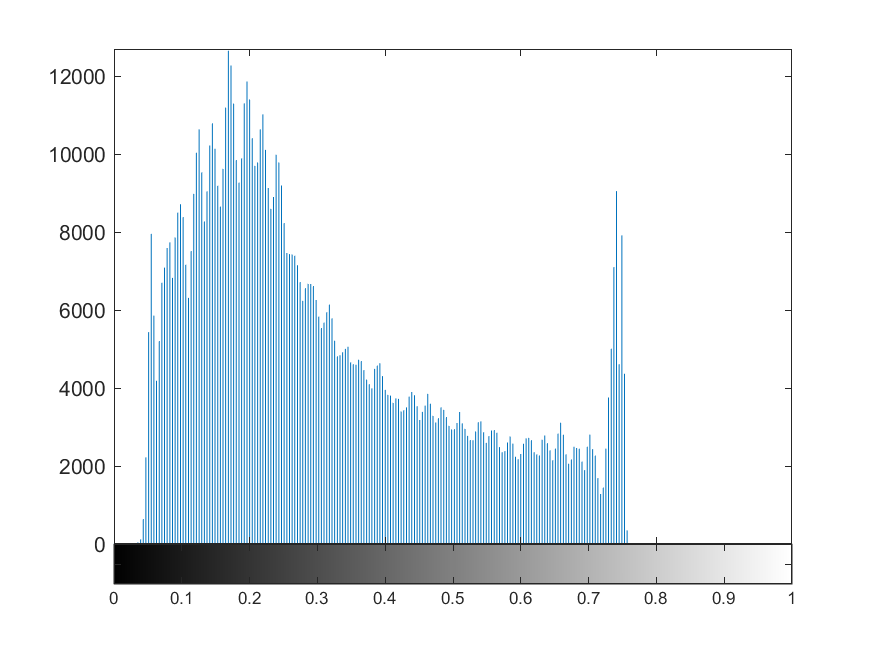
\includegraphics[width=\ww\linewidth]{../zad1/WithCut/I2/H_Origin.png}} \hfill%	
    \subfloat[H(HSc($\text{Ox}_\text{+b\&w}$ ,p1)) \\ k1 = 1 \\ k2 = 2.6407 \\ k3 = 1 \\ k4 = 0.30172 \\ min(I) = 0 \\ max(I) = 1 ]{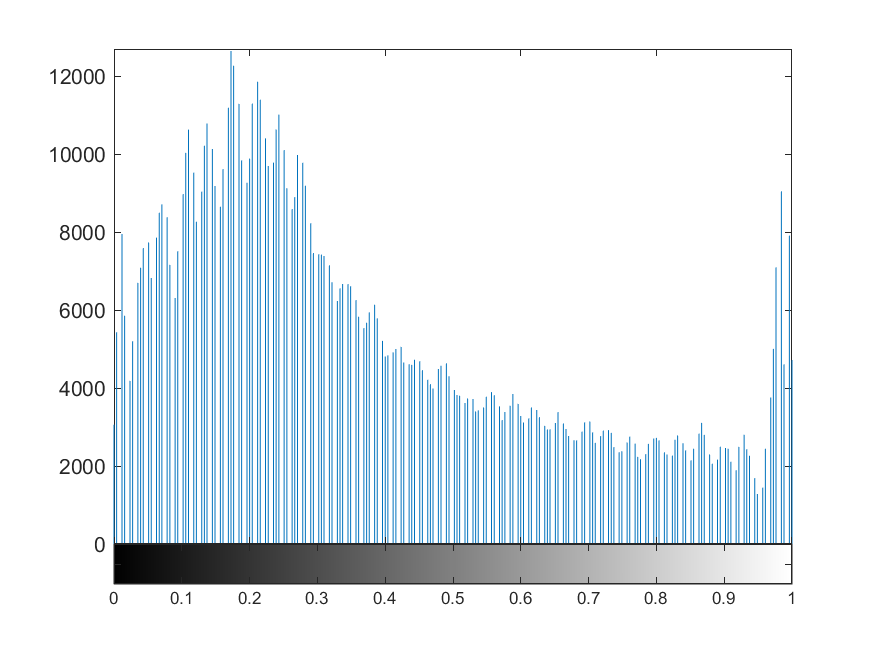
\includegraphics[width=\ww\linewidth]{../zad1/WithCut/I2/H_Cut_P1.png}} \hfill
    \subfloat[H(HSc($\text{Ox}_\text{+b\&w}$ ,p1)) \\ k1 = 1 \\ k2 = 2.6705 \\ k3 = 1 \\ k4 = 0.32133 \\ min(I) = 0 \\ max(I) = 1 ]{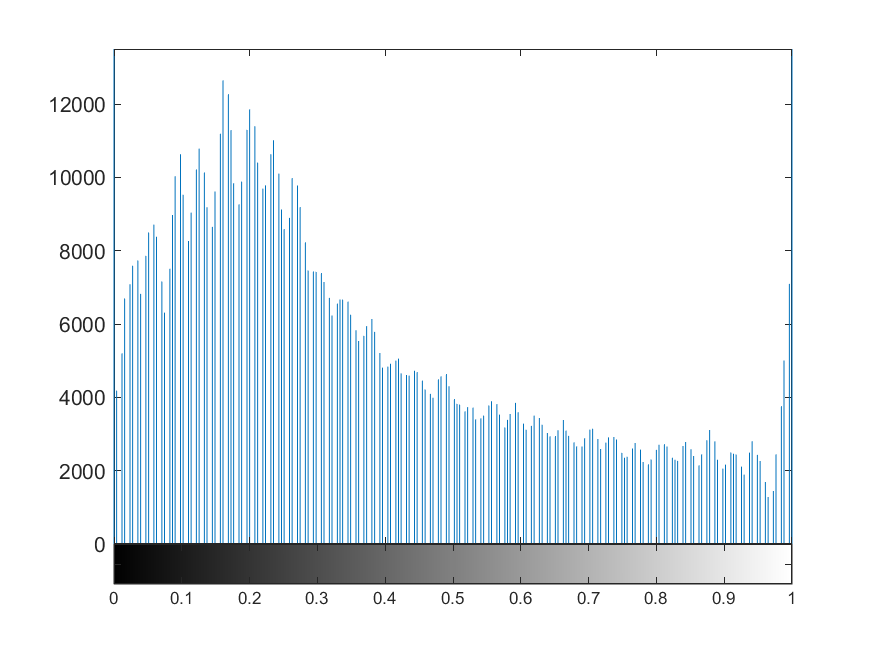
\includegraphics[width=\ww\linewidth]{../zad1/WithCut/I2/H_Cut_P2.png}} 
    \caption{Tekst do zmiany} 
    \label{fig:porownanie6}
\end{figure}

\begin{figure}[H]
    \captionsetup[subfloat]{justification=raggedright,singlelinecheck=false, position=bottom,labelformat=empty} %
    \subfloat[$\text{Ox}_\text{+b\&w}$                ]{\includegraphics[width=\ww\linewidth]{../zad1/WithCut/I3/I_Origin.png}} \hfill%	
    \subfloat[HSc($\text{Ox}_\text{+b\&w}$ ,p1)       ]{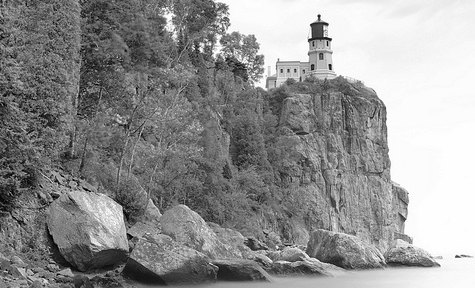
\includegraphics[width=\ww\linewidth]{../zad1/WithCut/I3/I_Cut_P1.png}} \hfill% wypełnenie
    \subfloat[HSc($\text{Ox}_\text{+b\&w}$ ,p1)       ]{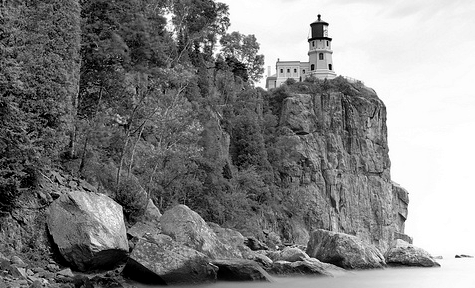
\includegraphics[width=\ww\linewidth]{../zad1/WithCut/I3/I_Cut_P2.png}} \\
    \subfloat[H($\text{Ox}_\text{+b\&w}$)          \\ k1 = 1 \\ k2 = 1.8045 \\ k3 = 1 \\ k4 = 0.16253 \\ min(I) = 0 \\ max(I) = 1 ]{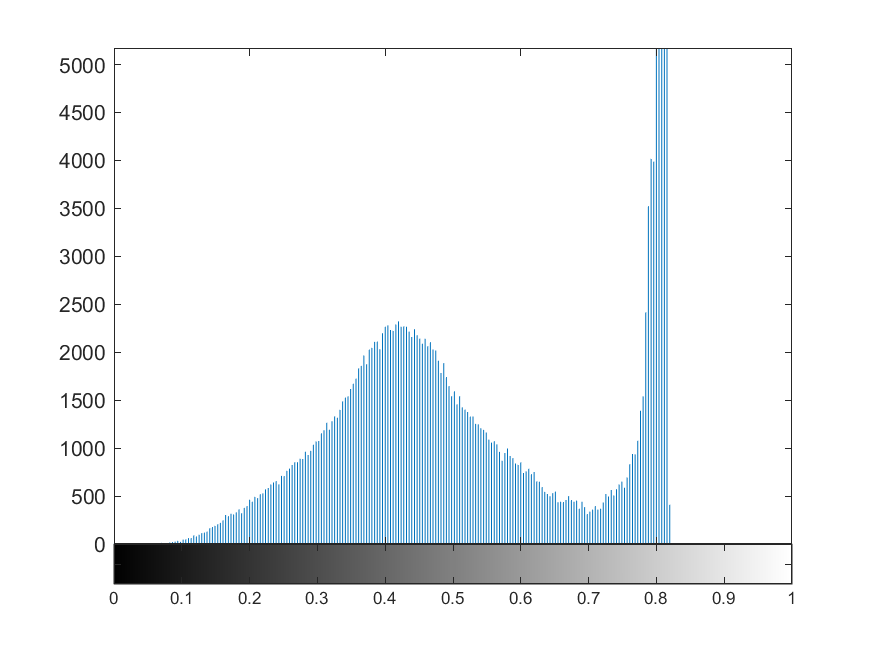
\includegraphics[width=\ww\linewidth]{../zad1/WithCut/I3/H_Origin.png}} \hfill%	
    \subfloat[H(HSc($\text{Ox}_\text{+b\&w}$ ,p1)) \\ k1 = 1 \\ k2 = 1.5869 \\ k3 = 1 \\ k4 = 0.3154 \\ min(I) = 0 \\ max(I) = 1 ]{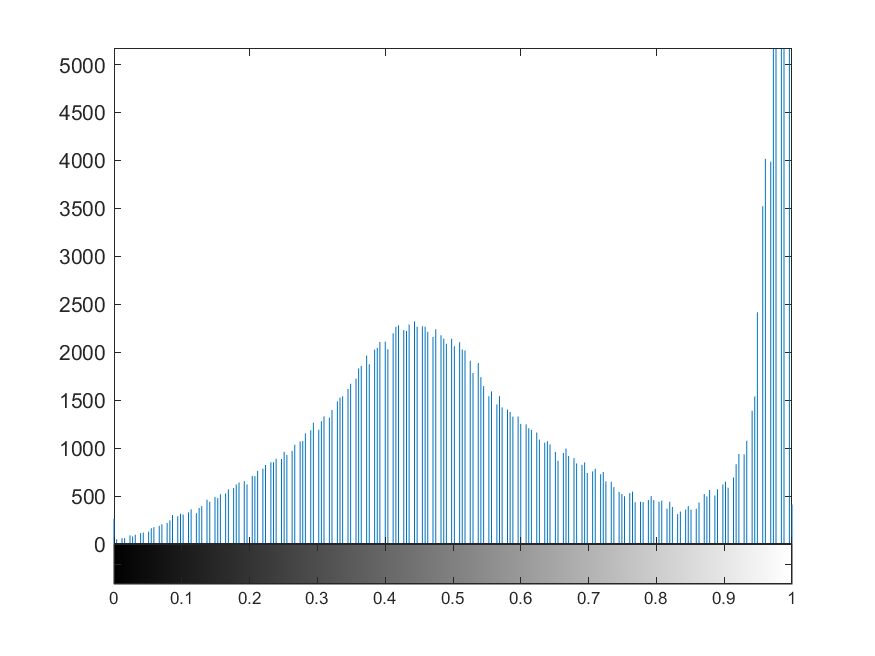
\includegraphics[width=\ww\linewidth]{../zad1/WithCut/I3/H_Cut_P1.png}} \hfill
    \subfloat[H(HSc($\text{Ox}_\text{+b\&w}$ ,p1)) \\ k1 = 1 \\ k2 = 1.7267 \\ k3 = 1 \\ k4 = 0.41726 \\ min(I) = 0 \\ max(I) = 1 ]{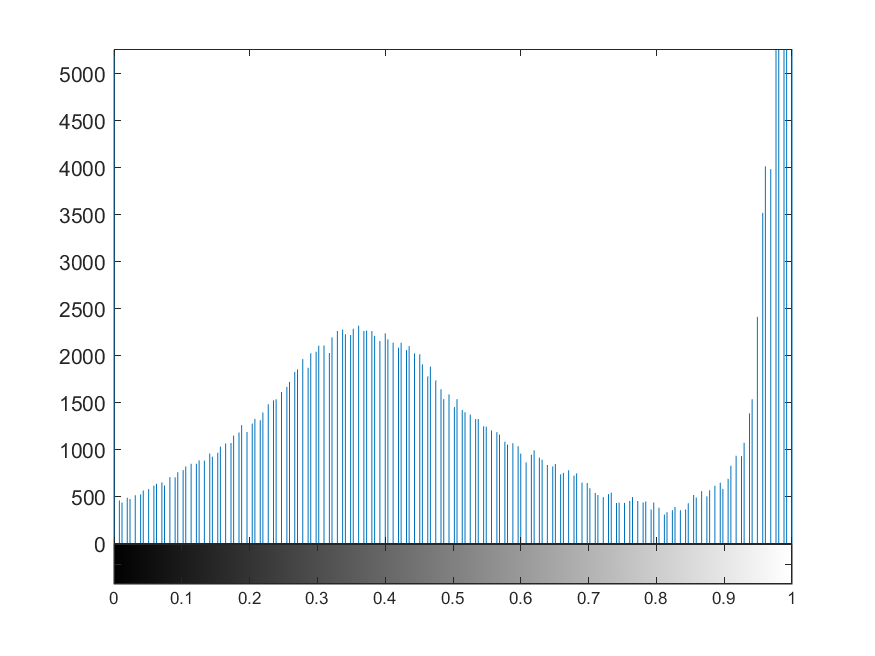
\includegraphics[width=\ww\linewidth]{../zad1/WithCut/I3/H_Cut_P2.png}} 
    \caption{Tekst do zmiany} 
    \label{fig:porownanie7}
\end{figure}

\begin{figure}[H]
    \captionsetup[subfloat]{justification=raggedright,singlelinecheck=false, position=bottom,labelformat=empty} %
    \subfloat[$\text{Ox}_\text{+b\&w}$                ]{\includegraphics[width=\ww\linewidth]{../zad1/WithCut/I4/I_Origin.png}} \hfill%	
    \subfloat[HSc($\text{Ox}_\text{+b\&w}$ ,p1)       ]{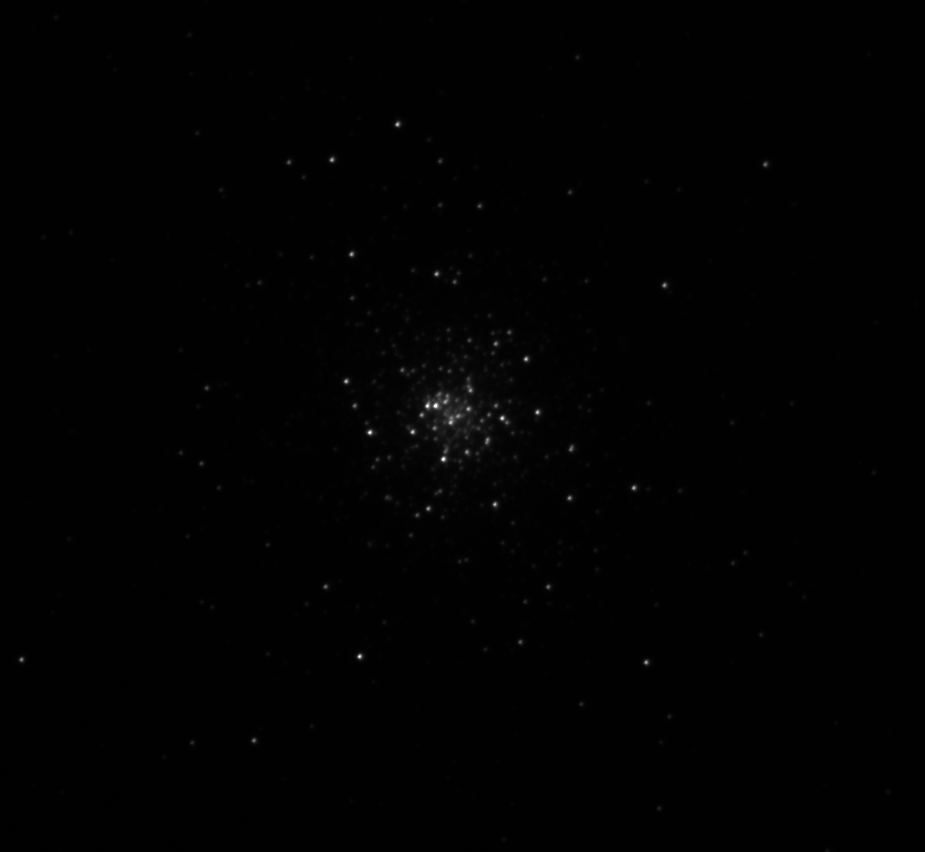
\includegraphics[width=\ww\linewidth]{../zad1/WithCut/I4/I_Cut_P1.png}} \hfill% wypełnenie
    \subfloat[HSc($\text{Ox}_\text{+b\&w}$ ,p1)       ]{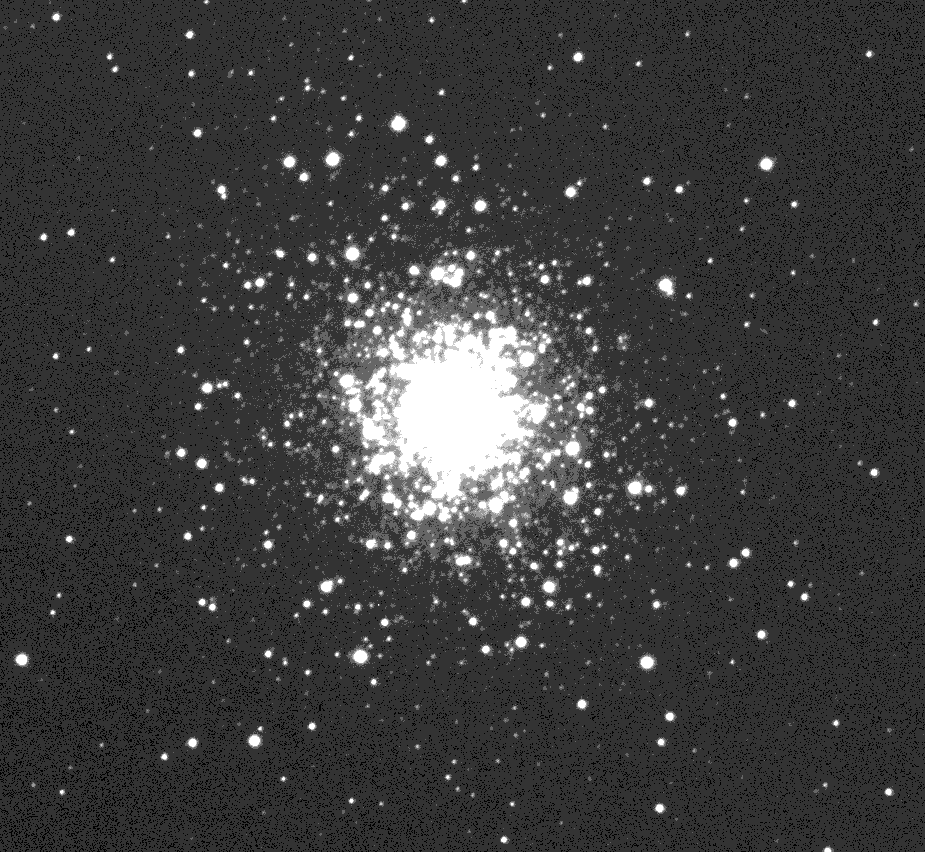
\includegraphics[width=\ww\linewidth]{../zad1/WithCut/I4/I_Cut_P2.png}} \\
    \subfloat[H($\text{Ox}_\text{+b\&w}$)          \\ k1 = 1 \\ k2 = 31.566 \\ k3 = 1 \\ k4 = 0.013199 \\ min(I) = 0 \\ max(I) = 1 ]{\includegraphics[width=\ww\linewidth]{../zad1/WithCut/I4/H_Origin.png}} \hfill%	
    \subfloat[H(HSc($\text{Ox}_\text{+b\&w}$ ,p1)) \\ k1 = 1 \\ k2 = 119.81 \\ k3 = 1 \\ k4 = 0.013842 \\ min(I) = 0 \\ max(I) = 1 ]{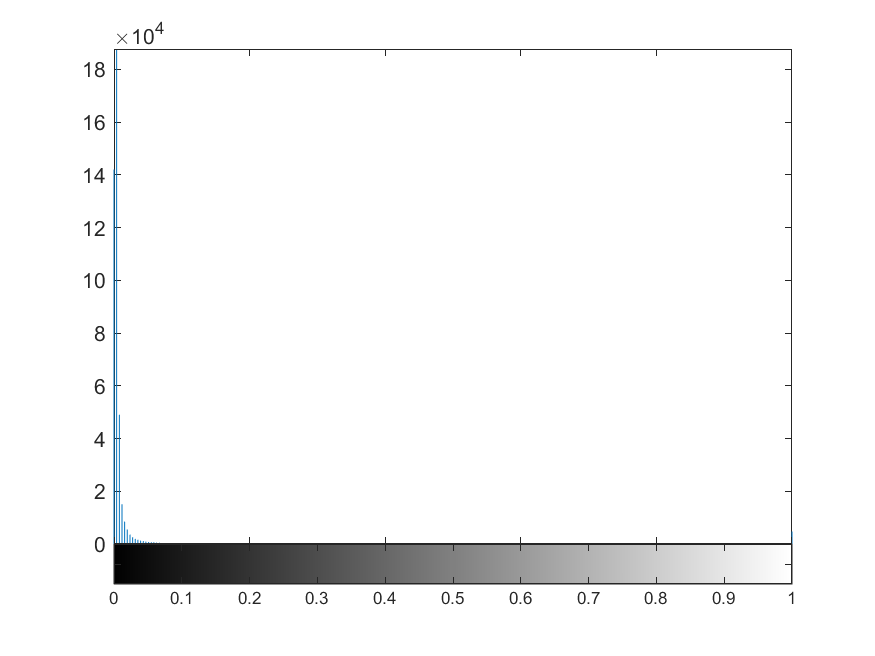
\includegraphics[width=\ww\linewidth]{../zad1/WithCut/I4/H_Cut_P1.png}} \hfill
    \subfloat[H(HSc($\text{Ox}_\text{+b\&w}$ ,p1)) \\ k1 = 1 \\ k2 = 4.6968 \\ k3 = 1 \\ k4 = 0.093701 \\ min(I) = 0 \\ max(I) = 1 ]{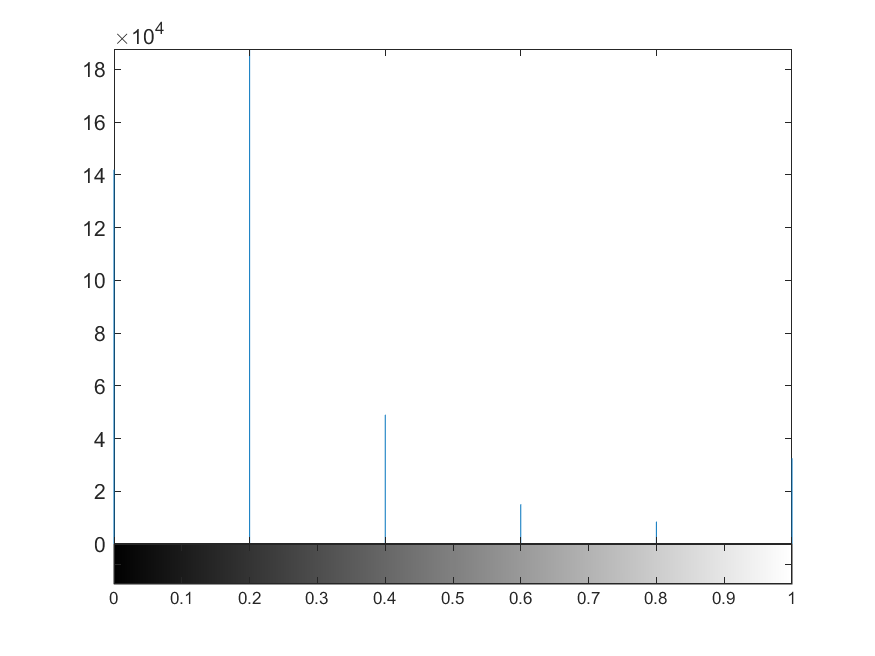
\includegraphics[width=\ww\linewidth]{../zad1/WithCut/I4/H_Cut_P2.png}} 
    \caption{Tekst do zmiany} 
    \label{fig:porownanie8}
\end{figure}



\section*{Zadanie 2. Lokalna poprawa histogramu}
\subsection*{Metoda własna}

\begin{figure}[H]
    \captionsetup[subfloat]{justification=raggedright,singlelinecheck=false, position=bottom,labelformat=empty} %
    \subfloat[Ox           ]{\includegraphics[width=\ww\linewidth]{../zad2/Local/I1/I_Origin.png}} \hfill%	
    \subfloat[MG(Ox)       ]{\includegraphics[width=\ww\linewidth]{../zad2/Local/I1/I_Global.png}} \hfill% wypełnenie
    \subfloat[ML(Ox)       ]{\includegraphics[width=\ww\linewidth]{../zad2/Local/I1/I_LocalF.png}} \\
    \subfloat[H(Ox)     \\ k1 = 0.28627 \\ k2 = 2.3275 \\ k3 = 1 \\ k4 = 0.010884 \\ min(I) = 0 \\ max(I) = 0.28627 ]{\includegraphics[width=\ww\linewidth]{../zad2/Local/I1/H_Origin.png}} \hfill%	
    \subfloat[H(MG(Ox)) \\ k1 = 1 \\ k2 = 2.3834 \\ k3 = 1 \\ k4 = 0.20638 \\ min(I) = 0 \\ max(I) = 1 ]{\includegraphics[width=\ww\linewidth]{../zad2/Local/I1/H_Global.png}} \hfill
    \subfloat[H(ML(Ox)) \\ k1 = 1 \\ k2 = 2.3625 \\ k3 = 1 \\ k4 = 0.17425 \\ min(I) = 0 \\ max(I) = 1 ]{\includegraphics[width=\ww\linewidth]{../zad2/Local/I1/H_LocalF.png}} 
    \caption{Tekst do zmiany} 
    \label{fig:porownanie9}
\end{figure}

\begin{figure}[H]
    \captionsetup[subfloat]{justification=raggedright,singlelinecheck=false, position=bottom,labelformat=empty} %
    \subfloat[Ox           ]{\includegraphics[width=\ww\linewidth]{../zad2/Local/I2/I_Origin.png}} \hfill%	
    \subfloat[MG(Ox)       ]{\includegraphics[width=\ww\linewidth]{../zad2/Local/I2/I_Global.png}} \hfill% wypełnenie
    \subfloat[ML(Ox)       ]{\includegraphics[width=\ww\linewidth]{../zad2/Local/I2/I_LocalF.png}} \\
    \subfloat[H(Ox)     \\ k1 = 0.76078 \\ k2 = 2.4201 \\ k3 = 1 \\ k4 = 0.15035 \\ min(I) = 0 \\ max(I) = 0.76078 ]{\includegraphics[width=\ww\linewidth]{../zad2/Local/I2/H_Origin.png}} \hfill%	
    \subfloat[H(MG(Ox)) \\ k1 = 1 \\ k2 = 2.6749 \\ k3 = 1 \\ k4 = 0.31168 \\ min(I) = 0 \\ max(I) = 1 ]{\includegraphics[width=\ww\linewidth]{../zad2/Local/I2/H_Global.png}} \hfill
    \subfloat[H(ML(Ox)) \\ k1 = 1 \\ k2 = 2.357 \\ k3 = 1 \\ k4 = 0.27598 \\ min(I) = 0 \\ max(I) = 1 ]{\includegraphics[width=\ww\linewidth]{../zad2/Local/I2/H_LocalF.png}} 
    \caption{Tekst do zmiany} 
    \label{fig:porownanie10}
\end{figure}

\begin{figure}[H]
    \captionsetup[subfloat]{justification=raggedright,singlelinecheck=false, position=bottom,labelformat=empty} %
    \subfloat[Ox           ]{\includegraphics[width=\ww\linewidth]{../zad2/Local/I3/I_Origin.png}} \hfill%	
    \subfloat[MG(Ox)       ]{\includegraphics[width=\ww\linewidth]{../zad2/Local/I3/I_Global.png}} \hfill% wypełnenie
    \subfloat[ML(Ox)       ]{\includegraphics[width=\ww\linewidth]{../zad2/Local/I3/I_LocalF.png}} \\
    \subfloat[H(Ox)     \\ k1 = 0.81961 \\ k2 = 1.479 \\ k3 = 1 \\ k4 = 0.16253 \\ min(I) = 0 \\ max(I) = 0.81961 ]{\includegraphics[width=\ww\linewidth]{../zad2/Local/I3/H_Origin.png}} \hfill%	
    \subfloat[H(MG(Ox)) \\ k1 = 1 \\ k2 = 1.6703 \\ k3 = 1 \\ k4 = 0.38127 \\ min(I) = 0 \\ max(I) = 1 ]{\includegraphics[width=\ww\linewidth]{../zad2/Local/I3/H_Global.png}} \hfill
    \subfloat[H(ML(Ox)) \\ k1 = 1 \\ k2 = 1.6713 \\ k3 = 1 \\ k4 = 0.22355 \\ min(I) = 0 \\ max(I) = 1 ]{\includegraphics[width=\ww\linewidth]{../zad2/Local/I3/H_LocalF.png}} 
    \caption{Tekst do zmiany} 
    \label{fig:porownanie11}
\end{figure}

\begin{figure}[H]
    \captionsetup[subfloat]{justification=raggedright,singlelinecheck=false, position=bottom,labelformat=empty} %
    \subfloat[Ox           ]{\includegraphics[width=\ww\linewidth]{../zad2/Local/I4/I_Origin.png}} \hfill%	
    \subfloat[MG(Ox)       ]{\includegraphics[width=\ww\linewidth]{../zad2/Local/I4/I_Global.png}} \hfill% wypełnenie
    \subfloat[ML(Ox)       ]{\includegraphics[width=\ww\linewidth]{../zad2/Local/I4/I_LocalF.png}} \\
    \subfloat[H(Ox)     \\ k1 = 0.99216 \\ k2 = 31.319 \\ k3 = 0.98444 \\ k4 = 0.013196 \\ min(I) = 0.0078431 \\ max(I) = 1 ]{\includegraphics[width=\ww\linewidth]{../zad2/Local/I4/H_Origin.png}} \hfill%	
    \subfloat[H(MG(Ox)) \\ k1 = 1 \\ k2 = 10.334 \\ k3 = 1 \\ k4 = 0.053817 \\ min(I) = 0 \\ max(I) = 1 ]{\includegraphics[width=\ww\linewidth]{../zad2/Local/I4/H_Global.png}} \hfill
    \subfloat[H(ML(Ox)) \\ k1 = 1 \\ k2 = 10.275 \\ k3 = 1 \\ k4 = 0.044515 \\ min(I) = 0 \\ max(I) = 1 ]{\includegraphics[width=\ww\linewidth]{../zad2/Local/I4/H_LocalF.png}} 
    \caption{Tekst do zmiany} 
    \label{fig:porownanie12}
\end{figure}



\subsection*{Metoda CLAHE}


\begin{figure}[H]
    \captionsetup[subfloat]{justification=raggedright,singlelinecheck=false, position=bottom,labelformat=empty} %
    \subfloat[Ox                 ]{\includegraphics[width=\ww\linewidth]{../zad2/Clahe/I1/I_Origin.png}} \hfill%	
    \subfloat[CLAHE(Ox,p1)       ]{\includegraphics[width=\ww\linewidth]{../zad2/Clahe/I1/I_CLAHE1.png}} \hfill% wypełnenie
    \subfloat[CLAHE(Ox,p2)       ]{\includegraphics[width=\ww\linewidth]{../zad2/Clahe/I1/I_CLAHE2.png}} \\
    \subfloat[H(Ox)           \\ k1 = 0.28627 \\ k2 = 2.3275 \\ k3 = 1 \\ k4 = 0.010884 \\ min(I) = 0 \\ max(I) = 0.28627 ]{\includegraphics[width=\ww\linewidth]{../zad2/Clahe/I1/H_Origin.png}} \hfill%	
    \subfloat[H(CLAHE(Ox,p1)) \\ k1 = 0.57974 \\ k2 = 2.6299 \\ k3 = 0.9919 \\ k4 = 0.045114 \\ min(I) = 0.0023668 \\ max(I) = 0.5821 ]{\includegraphics[width=\ww\linewidth]{../zad2/Clahe/I1/H_CLAHE1.png}} \hfill
    \subfloat[H(CLAHE(Ox,p2)) \\ k1 = 0.79676 \\ k2 = 2.7165 \\ k3 = 0.99578 \\ k4 = 0.094358 \\ min(I) = 0.0016876 \\ max(I) = 0.79844 ]{\includegraphics[width=\ww\linewidth]{../zad2/Clahe/I1/H_CLAHE2.png}} 
    \caption{Tekst do zmiany} 
    \label{fig:porownanie13}
\end{figure}

\begin{figure}[H]
    \captionsetup[subfloat]{justification=raggedright,singlelinecheck=false, position=bottom,labelformat=empty} %
    \subfloat[Ox                 ]{\includegraphics[width=\ww\linewidth]{../zad2/Clahe/I2/I_Origin.png}} \hfill%	
    \subfloat[CLAHE(Ox,p1)       ]{\includegraphics[width=\ww\linewidth]{../zad2/Clahe/I2/I_CLAHE1.png}} \hfill% wypełnenie
    \subfloat[CLAHE(Ox,p2)       ]{\includegraphics[width=\ww\linewidth]{../zad2/Clahe/I2/I_CLAHE2.png}} \\
    \subfloat[H(Ox)           \\ k1 = 0.76078 \\ k2 = 2.4201 \\ k3 = 1 \\ k4 = 0.15035 \\ min(I) = 0 \\ max(I) = 0.76078 ]{\includegraphics[width=\ww\linewidth]{../zad2/Clahe/I2/H_Origin.png}} \hfill%	
    \subfloat[H(CLAHE(Ox,p1)) \\ k1 = 0.95151 \\ k2 = 2.5082 \\ k3 = 0.99577 \\ k4 = 0.21578 \\ min(I) = 0.0020192 \\ max(I) = 0.95353 ]{\includegraphics[width=\ww\linewidth]{../zad2/Clahe/I2/H_CLAHE1.png}} \hfill
    \subfloat[H(CLAHE(Ox,p2)) \\ k1 = 0.99447 \\ k2 = 2.3645 \\ k3 = 0.99748 \\ k4 = 0.23846 \\ min(I) = 0.0012567 \\ max(I) = 0.99573 ]{\includegraphics[width=\ww\linewidth]{../zad2/Clahe/I2/H_CLAHE2.png}} 
    \caption{Tekst do zmiany} 
    \label{fig:porownanie14}
\end{figure}

\begin{figure}[H]
    \captionsetup[subfloat]{justification=raggedright,singlelinecheck=false, position=bottom,labelformat=empty} %
    \subfloat[Ox                 ]{\includegraphics[width=\ww\linewidth]{../zad2/Clahe/I3/I_Origin.png}} \hfill%	
    \subfloat[CLAHE(Ox,p1)       ]{\includegraphics[width=\ww\linewidth]{../zad2/Clahe/I3/I_CLAHE1.png}} \hfill% wypełnenie
    \subfloat[CLAHE(Ox,p2)       ]{\includegraphics[width=\ww\linewidth]{../zad2/Clahe/I3/I_CLAHE2.png}} \\
    \subfloat[H(Ox)           \\ k1 = 0.81961 \\ k2 = 1.479 \\ k3 = 1 \\ k4 = 0.16253 \\ min(I) = 0 \\ max(I) = 0.81961 ]{\includegraphics[width=\ww\linewidth]{../zad2/Clahe/I3/H_Origin.png}} \hfill%	
    \subfloat[H(CLAHE(Ox,p1)) \\ k1 = 0.99521 \\ k2 = 1.6703 \\ k3 = 0.99749 \\ k4 = 0.21008 \\ min(I) = 0.00125 \\ max(I) = 0.99646 ]{\includegraphics[width=\ww\linewidth]{../zad2/Clahe/I3/H_CLAHE1.png}} \hfill
    \subfloat[H(CLAHE(Ox,p2)) \\ k1 = 0.99949 \\ k2 = 1.6616 \\ k3 = 0.99905 \\ k4 = 0.24875 \\ min(I) = 0.000475 \\ max(I) = 0.99996 ]{\includegraphics[width=\ww\linewidth]{../zad2/Clahe/I3/H_CLAHE2.png}} 
    \caption{Tekst do zmiany} 
    \label{fig:porownanie15}
\end{figure}

\begin{figure}[H]
    \captionsetup[subfloat]{justification=raggedright,singlelinecheck=false, position=bottom,labelformat=empty} %
    \subfloat[Ox                 ]{\includegraphics[width=\ww\linewidth]{../zad2/Clahe/I4/I_Origin.png}} \hfill%	
    \subfloat[CLAHE(Ox,p1)       ]{\includegraphics[width=\ww\linewidth]{../zad2/Clahe/I4/I_CLAHE1.png}} \hfill% wypełnenie
    \subfloat[CLAHE(Ox,p2)       ]{\includegraphics[width=\ww\linewidth]{../zad2/Clahe/I4/I_CLAHE2.png}} \\
    \subfloat[H(Ox)           \\ k1 = 0.99216 \\ k2 = 31.319 \\ k3 = 0.98444 \\ k4 = 0.013196 \\ min(I) = 0.0078431 \\ max(I) = 1 ]{\includegraphics[width=\ww\linewidth]{../zad2/Clahe/I4/H_Origin.png}} \hfill%	
    \subfloat[H(CLAHE(Ox,p1)) \\ k1 = 0.98955 \\ k2 = 21.983 \\ k3 = 0.97932 \\ k4 = 0.013491 \\ min(I) = 0.010447 \\ max(I) = 1 ]{\includegraphics[width=\ww\linewidth]{../zad2/Clahe/I4/H_CLAHE1.png}} \hfill
    \subfloat[H(CLAHE(Ox,p2)) \\ k1 = 0.98992 \\ k2 = 18.124 \\ k3 = 0.98004 \\ k4 = 0.01379 \\ min(I) = 0.010082 \\ max(I) = 1 ]{\includegraphics[width=\ww\linewidth]{../zad2/Clahe/I4/H_CLAHE2.png}} 
    \caption{Tekst do zmiany} 
    \label{fig:porownanie16}
\end{figure}




\newpage \section*{Kody programów}

      


\subsection*{ zad1.m                }  \lstinputlisting[language=Octave]{ ../matlab/zad1.m                } \newpage
\subsection*{ zad2.m                }  \lstinputlisting[language=Octave]{ ../matlab/zad2.m                } \newpage
\subsection*{ cropImage.m           }  \lstinputlisting[language=Octave]{ ../matlab/cropImage.m           } \newpage
\subsection*{ HistogramStretch.m    }  \lstinputlisting[language=Octave]{ ../matlab/HistogramStretch.m    } \newpage
\subsection*{ LocalContrastFix.m    }  \lstinputlisting[language=Octave]{ ../matlab/LocalContrastFix.m    } \newpage
\subsection*{ LocalContrastFix2.m   }  \lstinputlisting[language=Octave]{ ../matlab/LocalContrastFix2.m   } \newpage
\subsection*{ k1.m                  }  \lstinputlisting[language=Octave]{ ../matlab/k1.m                  } \newpage
\subsection*{ k2.m                  }  \lstinputlisting[language=Octave]{ ../matlab/k2.m                  } \newpage
\subsection*{ k3.m                  }  \lstinputlisting[language=Octave]{ ../matlab/k3.m                  } \newpage
\subsection*{ k4.m                  }  \lstinputlisting[language=Octave]{ ../matlab/k4.m                  } \newpage






\end{document}